\section{Study}
\label{sec:study}
In order to measure the method coverage reached by an exploration tool in one application, there is the need to know how many methods there are in the application and how many methods were called during the exploration. To achieve that, the application developers could count the number of methods in their project and write log lines at the beginning of every method. After that, they will need to compile, run the exploration tool against their application, measure the number of methods that were called during the exploration and compute statistics.

With that in mind, this study consists of nearly the same stages, i. instrumentation, ii. exploration, iii. coverage analysis, iv. summarize, and v. compute statistics. The stages ii. and iii. were repeated 10 times for every application that was selected, that leaded to the iv. stage.

The different stages were completed as follow:

Stage i: The applications' instrumentation was made by using InstruAPK. It is an instrumentation tool developed mainly for this study. This tool uses APKTool, a known Java application that allows inverse engineering in Android apps, allowing applications' instrumentation without the need of recompiling their source code. APKTool decodes the apk and the result is the smali representation of the app source code, These smali files are analysed in order to find all the methods to be instrumented and then, the log code is injected at the very beginning of each method. Its important to notice that no external libraries methods are instrumented. InstruAPK only search for methods following the android project structure that uses the application package name to store the application source code.

Stage ii: The exploration was made by four different automatic exploration tools. two from the industry and two from the academic side. The first tool was Firebase Test Lab. it was selected for being widely used in industry and for also being a Google product. The second one, Monkey, was selected for being the most basic one and because it is also included in the SDK for developing Android Apps. The third one, Droidbot, was selected from the academic side. Droidbot has been a point of study for many researches. Many others tools have based their functionality on this tool. The last one is RIP, this tool was selected for being of special interest for us. It is our own exploration tool and is is currently an active project inside the Software Design Lab at University of Los Andes. 

Every tool was executed ten times per application, and every execution with a maximum time of 30 minutes. Some tools ended its exploration before the max time. 
The number of executions and the maximum time were arbitrary decisions that were made because of time limitations for the study. Although, during the study was notice that most of the tools ended the exploration or reached their maximum coverage within the first 15 minutes. Which means that the maximum time for exploration was more than enough in almost all cases. 
 
stage iii: The coverage measurement was made by CoverageAnalyzer. It is a Java Application created mainly for this study. This tool analyses the resulting logcat of an Android phone, when executing an application that was instrumented by InstruAPK. It extracts different data such as, number of methods called, number of  methods never called, number of error traces of the application being analysed, most called methods, less called methods, as well as the time stamp of all calls of every method. It is important to notice that the possibility of extracting all those information is because InstruAPK provides it.

stage iv: Due to the multiple executions of every APK per tool, it is important to summarize de data. The final report contains the total number of unique methods called during all ten executions, reporting only the first time they were called.
The exploration reports are analysed and filtered as well.

stage v: This is the final stage of the study that involves, understanding data, computing statistics, creating graphs, extract insights and conclusions. 

Besides that, for this study, a set of 11 applications was used. This set is a subset of a set of open source applications utilised inside The Software Design Lab research group for other studies and tests, including RIP. Every APK in the subset should be successfully instrumented by InstruAPK, it should compile without any problem after instrumentation and it should be launch in an emulator without any issue after instrumentation.

\begin{figure}[h]
	\centering
	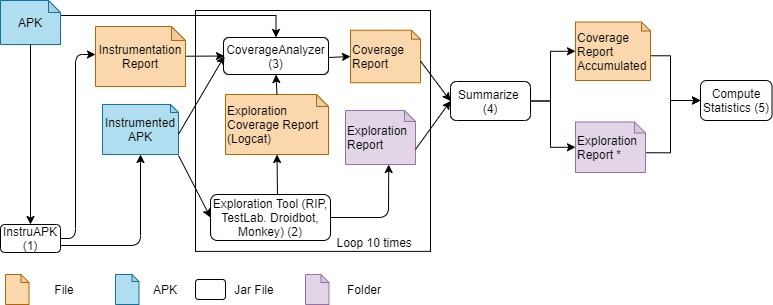
\includegraphics[width=0.5\textwidth]{img/workflow.jpg}
	\vspace{-0.5cm}
	\caption{Complete Study Workflow}
	\label{procesoTests}
\end{figure} 
